\noindent

\includegraphics[height=1.25cm]{images/pictograms/replication}

\includegraphics[height=1.25cm]{images/pictograms/benchmark}

\includegraphics[height=1.25cm]{images/pictograms/under_construction}

\includegraphics[height=1.25cm]{images/pictograms/FEM}
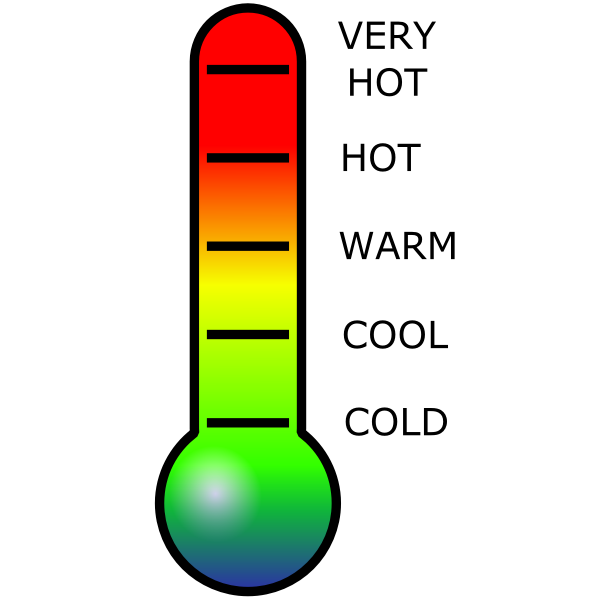
\includegraphics[height=1.25cm]{images/pictograms/temperature}

\includegraphics[height=1.25cm]{images/pictograms/paraview}

%%%%%%%%%%%%%%%%%%%%%%%%%%%%%%%%%%%%%%%%%%%%%%%%%%%%%%%%%%%%%%%%%%%%%%%%%%%%%%%%%%%%%%%%%%%%%%%%%%%

\begin{flushright} {\tiny {\color{gray} python\_codes/fieldstone\_173/text.tex}} \end{flushright}

%\lstinputlisting[language=bash,basicstyle=\small]{python_codes/template_keywords.key}

\par\noindent\rule{\textwidth}{0.4pt}

\begin{center}
\inpython
{\small Code: \url{https://github.com/cedrict/fieldstone/tree/master/python_codes/fieldstone_173}}
\end{center}

\par\noindent\rule{\textwidth}{0.4pt}

{\sl This stone was developed in collaboration with Donald Duck}. \index{contributors}{D. Duck}

\par\noindent\rule{\textwidth}{0.4pt}

Last revision: May. 23th, 2025.

\par\noindent\rule{\textwidth}{0.4pt}

%%%%%%%%%%%%%%%%%%%%%%%%%%%%%%%%%%%%%%%%%%%%%%%%%%%%%%%%%%%%%%%%%%%%%%%%%%%%%%%%%%%%%%%%%%%%%%%%%%%


\section*{Setup}

The domain is the unit square. 
The 2d steady state heat equation (with heat source) is solved, with $\rho=C_p=k=1$:
\[
\frac{\partial^2 T}{\partial x^2} + \frac{\partial^2 T}{\partial y^2} + S(x,y) = 0
\]
with $S(x,y)=-10$. 
The exact solution is 
\[
T(x,y)=(2x+y)^2
\]
since 
\[
\frac{\partial^2 T}{\partial x^2} + \frac{\partial^2 T}{\partial y^2}
= 2\cdot 2 \cdot 2 + 2 \cdot 1 \cdot 1 = 10
\]
The heat flux vector is then given by\footnote{the heat conductivity is equal to 1}
\[
\vec{q} = - \vec{\nabla} T = -2(2x+y) (2 \vec{e}_x + \vec{e}_y)
\]


We now turn to Figure 2 of the paper:
\begin{center}
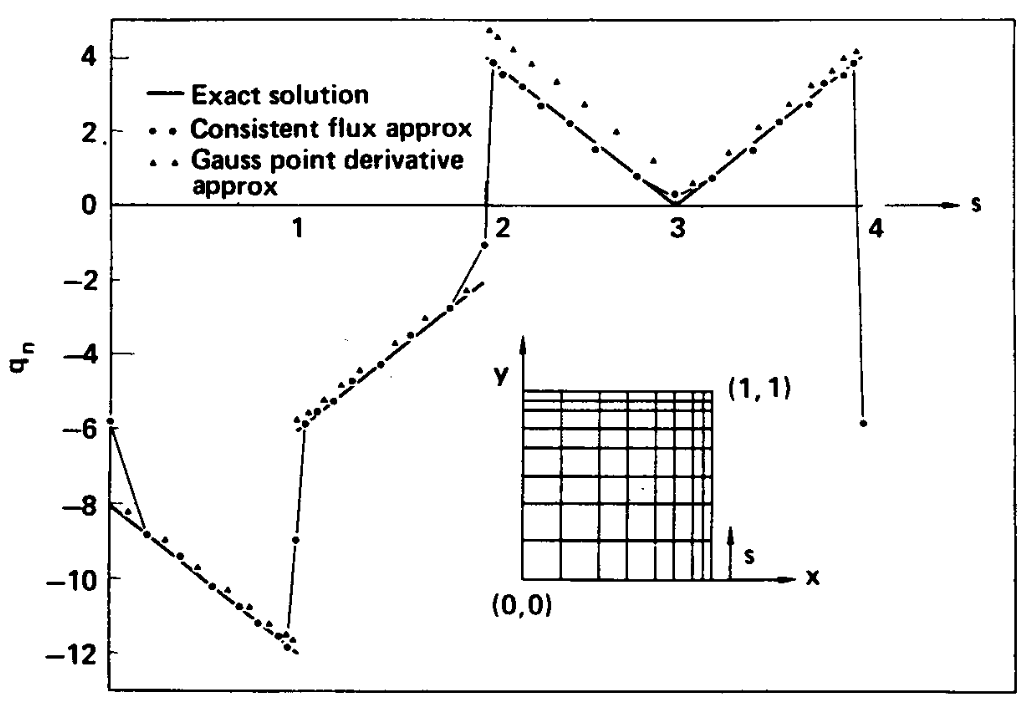
\includegraphics[width=7cm]{python_codes/fieldstone_173/images/grls87a}
\end{center}

We learn from it that the mesh counts $8\times 8$ elements with a gradual size change in space.
This is implemented as follows:
\begin{lstlisting}
for i in range(0,NV):
    x[i]=x[i]**0.66
    y[i]=y[i]**0.66
\end{lstlisting}

The mesh then looks like this:

\begin{center}
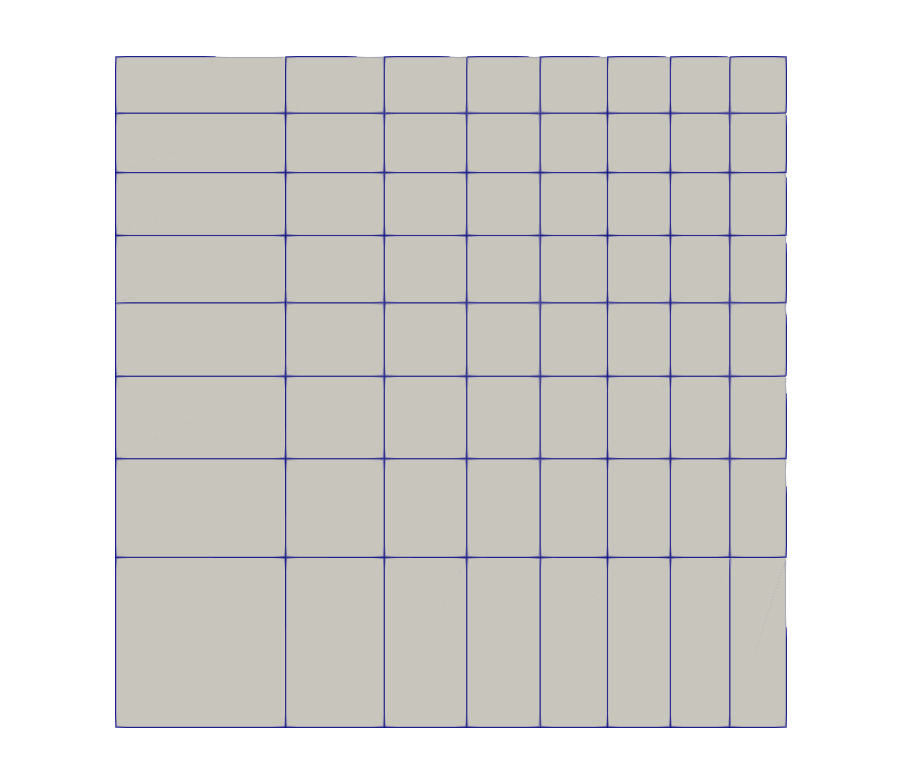
\includegraphics[width=7cm]{python_codes/fieldstone_173/images/mesh8x8}
\end{center}
This is not identical to the article but sufficiently close.


We then solve the equation on this mesh with $Q_1$ elements:

\begin{center}
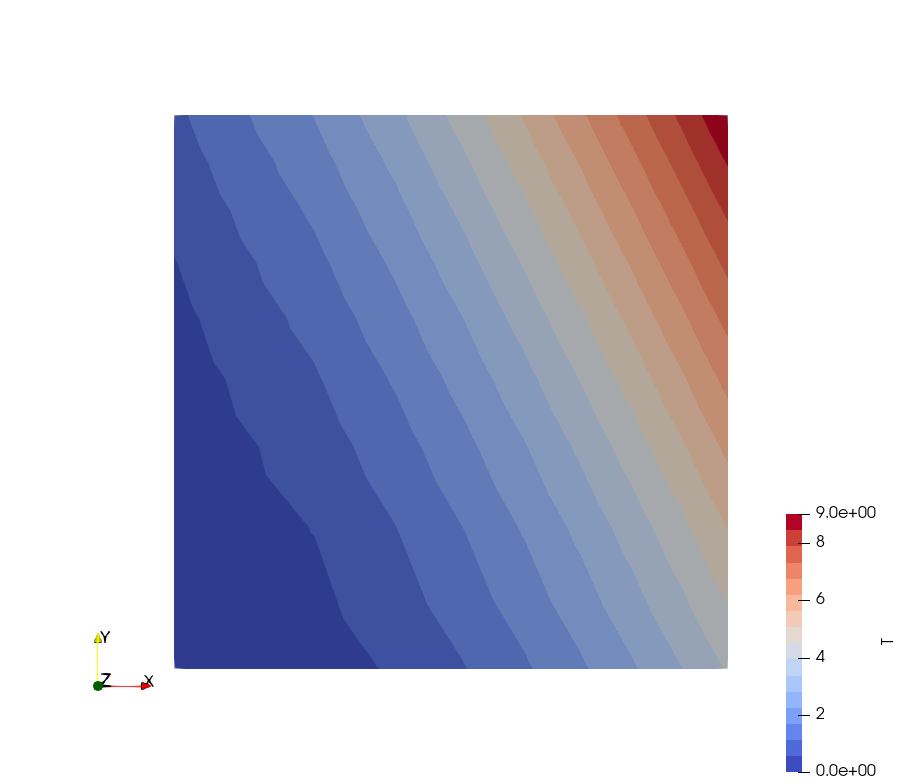
\includegraphics[width=5.7cm]{python_codes/fieldstone_173/results/T}
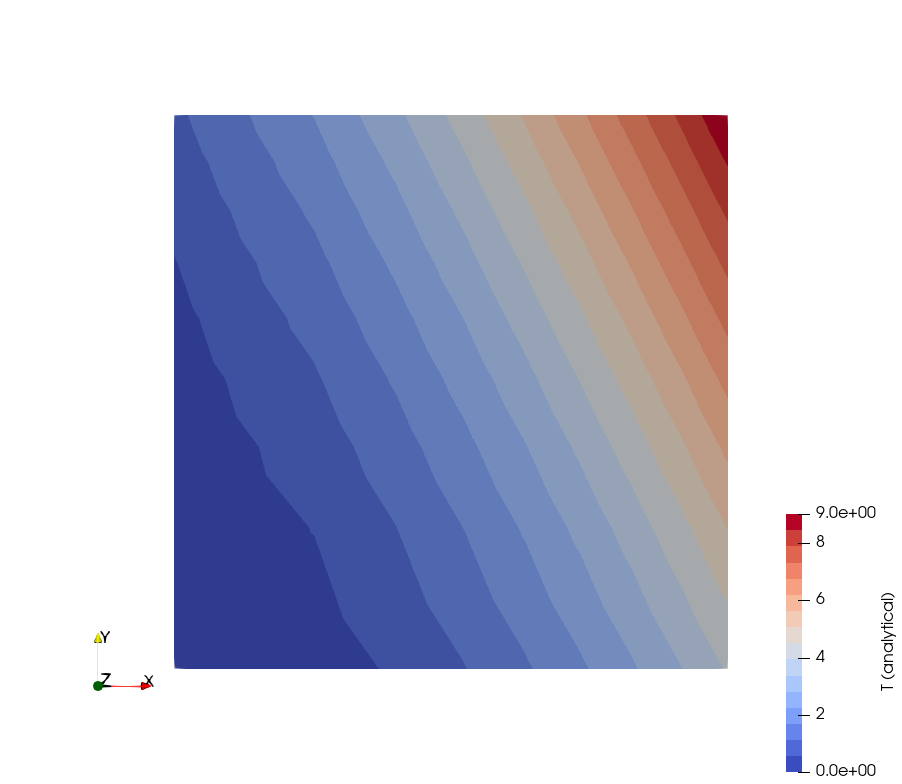
\includegraphics[width=5.7cm]{python_codes/fieldstone_173/results/T_analytical}
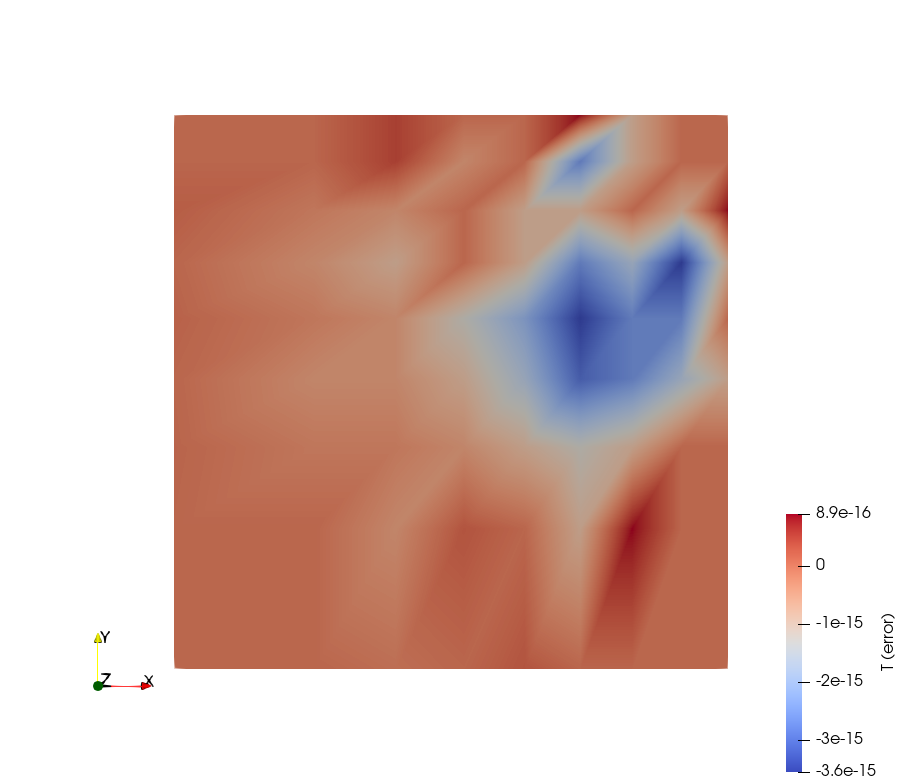
\includegraphics[width=5.7cm]{python_codes/fieldstone_173/results/T_error}\\
{\captionfont Temperature in the domain on stretched $8\times 8$ mesh. 
Left: computed; Middle: analytical; Right: error.}
\end{center}

We find that the calculated temperature is machine precision accurate.




%==============================================================================
\section*{Computing boundary normals}

Given the geometry of the domain, computing the normal to the boundary 
should not pose much problem. However, we need the normal vector at the nodes,
including the corner nodes. An inescapable question arises: 
what is the normal vector at the corners?

One option is to state that the problem is ill-posed and that the normal to a
singular point does not exist.

Another option is to look at the geometry of the domain (a rectangle), see that 
the corners then belong to two faces with normals orthogonal to each other 
and then set the normal vector to the average of the adjacent face normals.
For example the normal vector at point $(1,1)$ would then be $\vec{n}=(1,1)/\sqrt{2}$.

Finally, the last option is to follow the approach 
explained in \textcite{ensg82}: 
the normal vector at a node $i$ can be computed using the basis function derivatives:
\begin{eqnarray}
n_{x,i} &=& \frac{1}{n_i}\int_\Omega \frac{\partial \bN_i}{\partial x} dV \nn\\
n_{y,i} &=& \frac{1}{n_i}\int_\Omega \frac{\partial \bN_i}{\partial y} dV \nn
\end{eqnarray}
with 
\[
n_i = \left[
\left(\int_\Omega \frac{\partial \bN_i}{\partial x} dV\right)^2 +
\left(\int_\Omega \frac{\partial \bN_i}{\partial y} dV\right)^2 
\right]^{1/2}
\]

The integral over $\Omega$ is actually cheap: the nodes in question are on the boundary, 
and their basis functions have a compact support (on the boundary a node belongs to at 
most 2 elements) so that the code is as follows:

\begin{lstlisting}
nx=np.zeros(NV,dtype=np.float64) 
ny=np.zeros(NV,dtype=np.float64) 
jcb=np.zeros((ndim,ndim),dtype=np.float64)

for iel in range(0,nel):
    if surface_element[iel]: 
       for iq in range(0,nqperdim):
           for jq in range(0,nqperdim):

               rq=qcoords[iq]
               sq=qcoords[jq]
               weightq=qweights[iq]*qweights[jq]
               dNNNTdr=dNNTdr(rq,sq,order)
               dNNNTds=dNNTds(rq,sq,order)
               jcb[0,0]=np.dot(dNNNTdr[:],x[icon[:,iel]])
               jcb[0,1]=np.dot(dNNNTdr[:],y[icon[:,iel]])
               jcb[1,0]=np.dot(dNNNTds[:],x[icon[:,iel]])
               jcb[1,1]=np.dot(dNNNTds[:],y[icon[:,iel]])
               jcob = np.linalg.det(jcb)
               jcbi=np.linalg.inv(jcb)
               dNNNTdx=jcbi[0,0]*dNNNTdr[:]+jcbi[0,1]*dNNNTds[:]
               dNNNTdy=jcbi[1,0]*dNNNTdr[:]+jcbi[1,1]*dNNNTds[:]
               for k in range(0,m):
                   if boundary_node[icon[k,iel]]:
                      nx[icon[k,iel]]+=dNNNTdx[k]*jcob*weightq
                      ny[icon[k,iel]]+=dNNNTdy[k]*jcob*weightq
\end{lstlisting}
which is then followed by a normalisation:
\begin{lstlisting}
for i in range(0,NV):
    if boundary_node[i]:
       norm=np.sqrt(nx[i]**2+ny[i]**2)
       nx[i]/=norm
       ny[i]/=norm
\end{lstlisting}

In this case the normal vectors are as follows:
\begin{center}
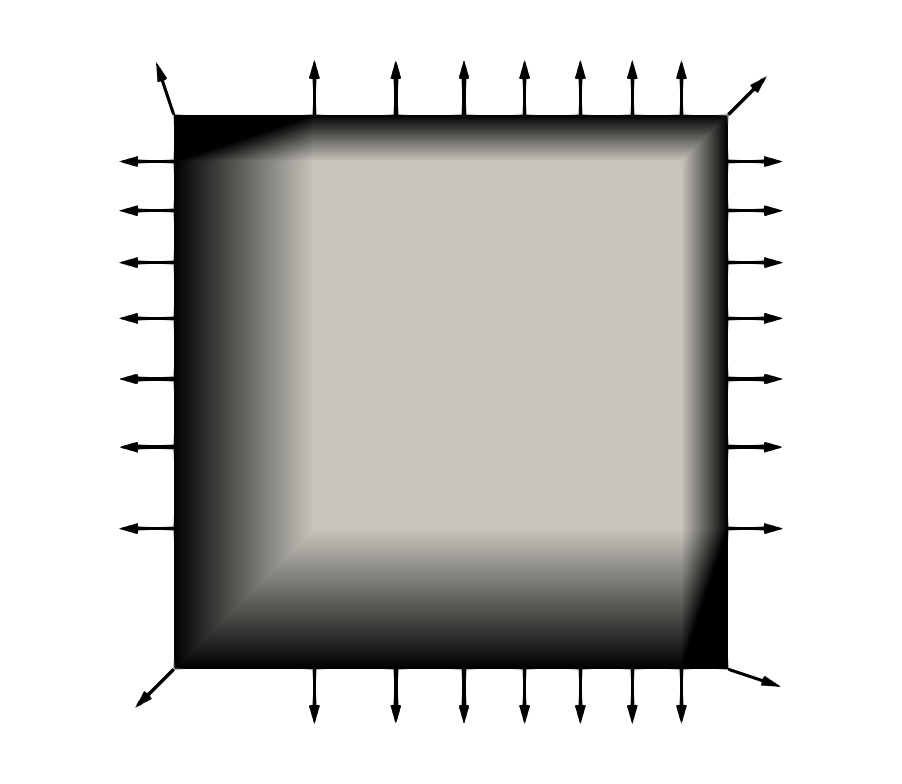
\includegraphics[width=5.7cm]{python_codes/fieldstone_173/results/normals}
\end{center}
We see that the vectors at the corners are not 'at $45$ degrees' if the element is not square.


%==============================================================================
\section*{Computing the nodal heat flux everywhere - method 1}

We apply here a standard technique: the derivatives of the temperature 
are computed at each corner of the element by means of the basis functions
and then averaged out on the nodes.

\begin{lstlisting}
    qx=np.zeros(NV,dtype=np.float64) 
    qy=np.zeros(NV,dtype=np.float64) 
    qn=np.zeros(NV,dtype=np.float64) 
    cc=np.zeros(NV,dtype=np.float64) 
    for iel in range(0,nel):
        for k in range(0,m):
            rq=rnodes[k]
            sq=snodes[k]
            inode=icon[k,iel]
            cc[inode]+=1
            dNNNTdr=dNNTdr(rq,sq,order)
            dNNNTds=dNNTds(rq,sq,order)
            jcb=np.zeros((ndim,ndim),dtype=np.float64)
            jcb[0,0]=np.sum(dNNNTdr[:]*x[icon[:,iel]])
            jcb[0,1]=np.sum(dNNNTdr[:]*y[icon[:,iel]])
            jcb[1,0]=np.sum(dNNNTds[:]*x[icon[:,iel]])
            jcb[1,1]=np.sum(dNNNTds[:]*y[icon[:,iel]])
            jcbi=np.linalg.inv(jcb)
            dNNNTdx[:]=jcbi[0,0]*dNNNTdr[:]+jcbi[0,1]*dNNNTds[:]
            dNNNTdy[:]=jcbi[1,0]*dNNNTdr[:]+jcbi[1,1]*dNNNTds[:]
            qx[inode]-=np.sum(dNNNTdx[:]*T[icon[:,iel]])
            qy[inode]-=np.sum(dNNNTdy[:]*T[icon[:,iel]])
        #end for
    #end for
    qx/=cc
    qy/=cc
    qn[:]=qx[:]*nx[:]+qy[:]*ny[:]
\end{lstlisting}

We find that this technique yields an accurate heat flux inside the domain 
but not so much on the boundary:

\begin{center}
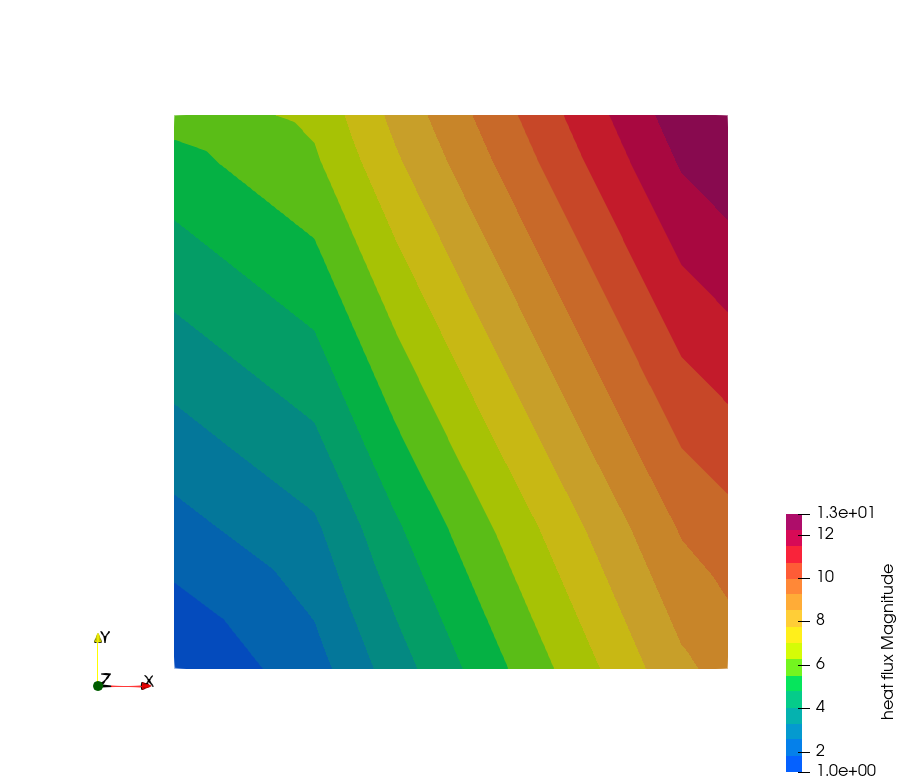
\includegraphics[width=5.7cm]{python_codes/fieldstone_173/results/q8}
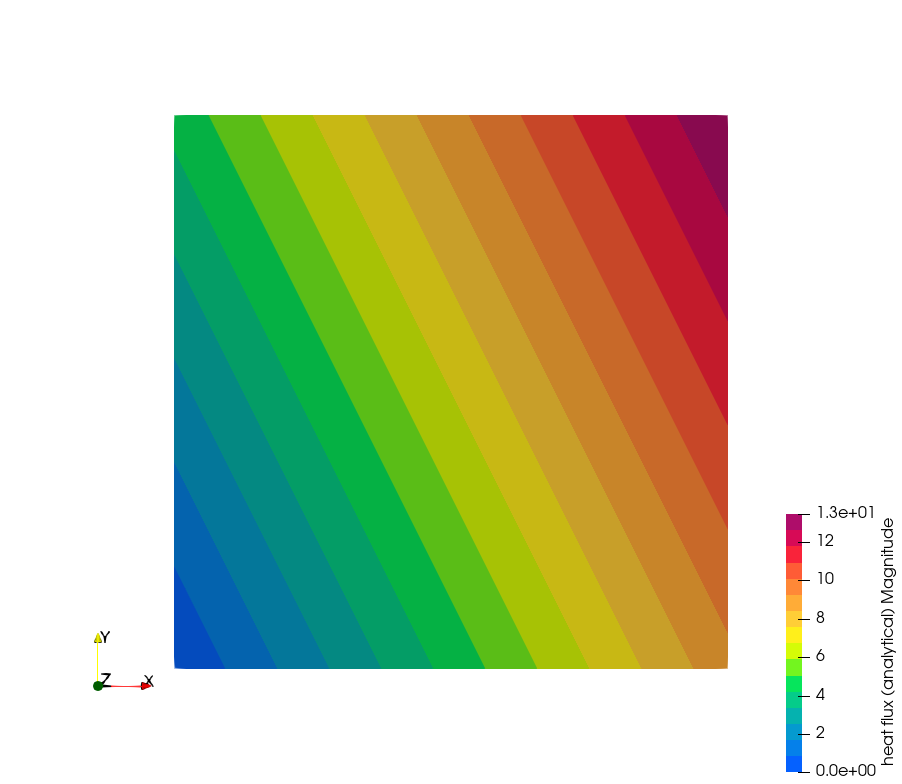
\includegraphics[width=5.7cm]{python_codes/fieldstone_173/results/q8_analytical}
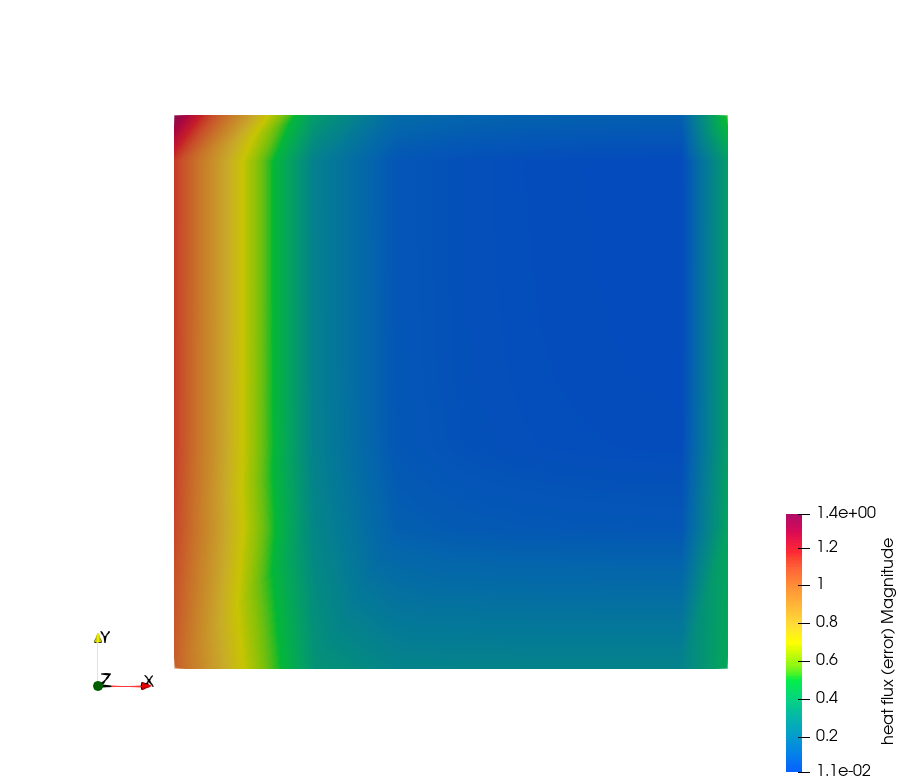
\includegraphics[width=5.7cm]{python_codes/fieldstone_173/results/q8_error}\\
{\captionfont Temperature in the domain on $8 \times 8$ mesh.}
\end{center}

We can also compute the heat flux on a higher resolution mesh:
\begin{center}
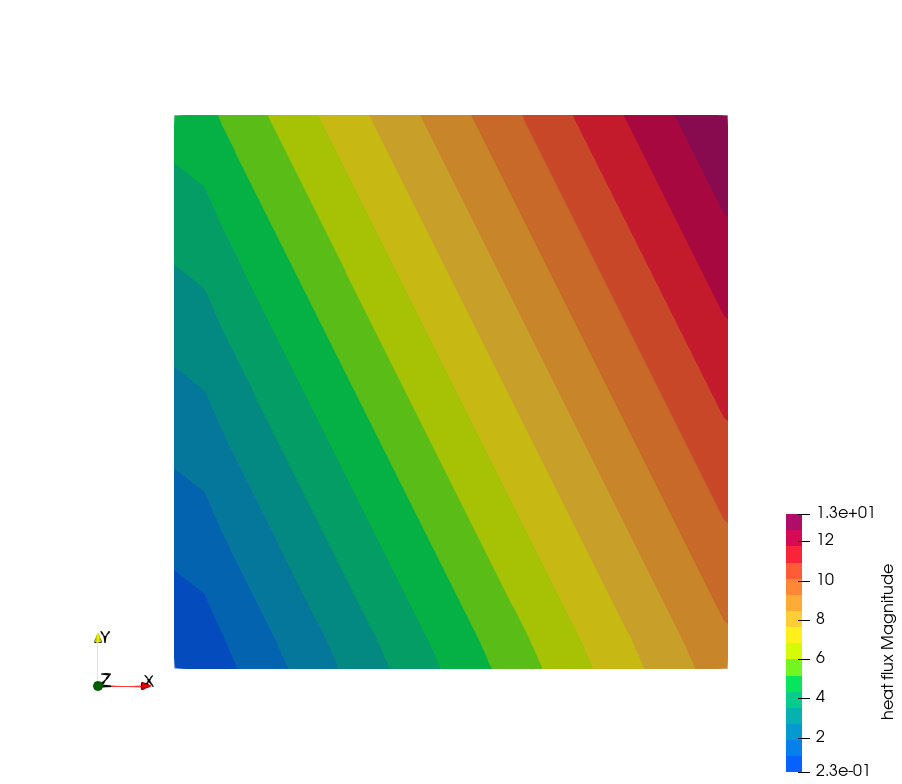
\includegraphics[width=5.7cm]{python_codes/fieldstone_173/results/q80}
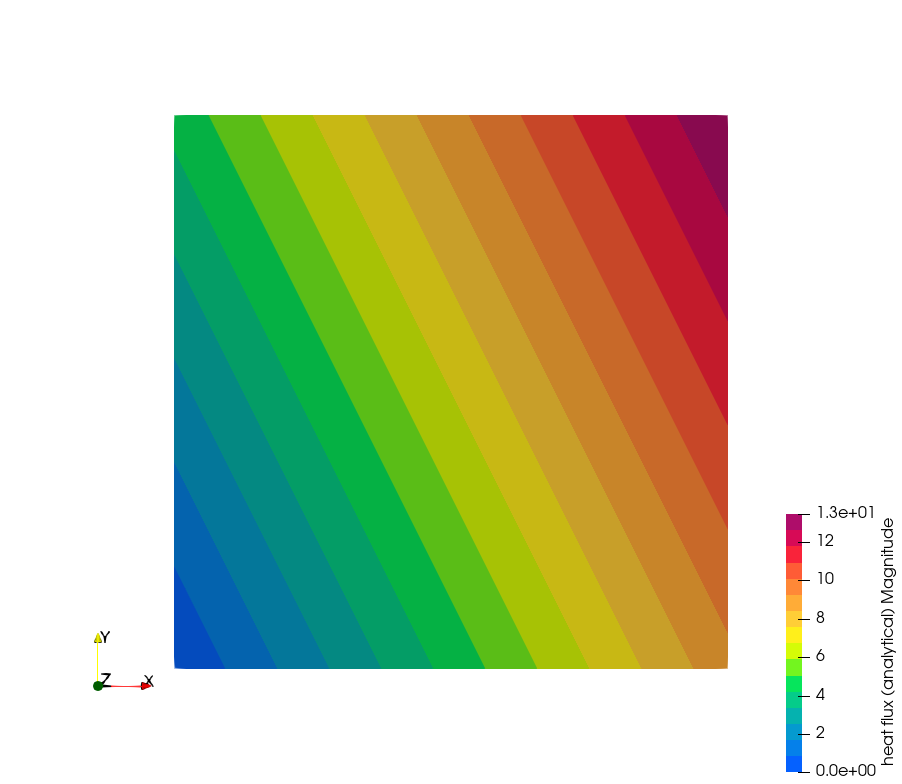
\includegraphics[width=5.7cm]{python_codes/fieldstone_173/results/q80_analytical}
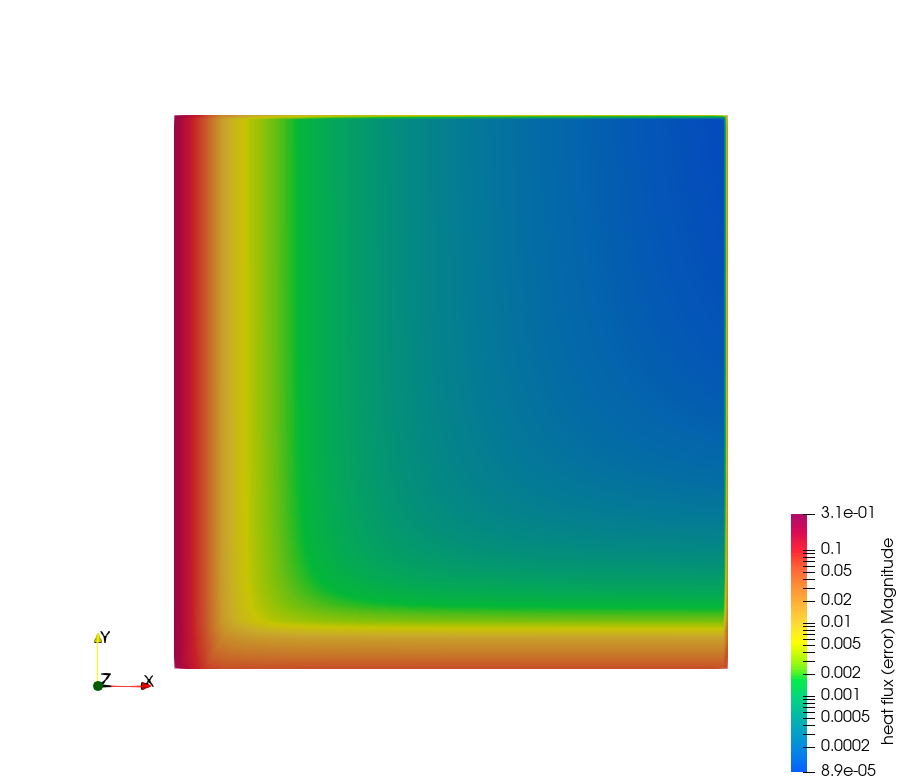
\includegraphics[width=5.7cm]{python_codes/fieldstone_173/results/q80_error}\\
{\captionfont Temperature in the domain on $80 \times 80$ mesh.}
\end{center}

In both cases we see that the heat flux is not accurate on the boundary.
As in \textcite{grls87} we can plot the normal heat flux, i.e. $q_n=\vec{q}\cdot \vec{n}$
along the boundary starting a the SE corner, moving to NE, then NW, then SW back to SE:

\begin{center}
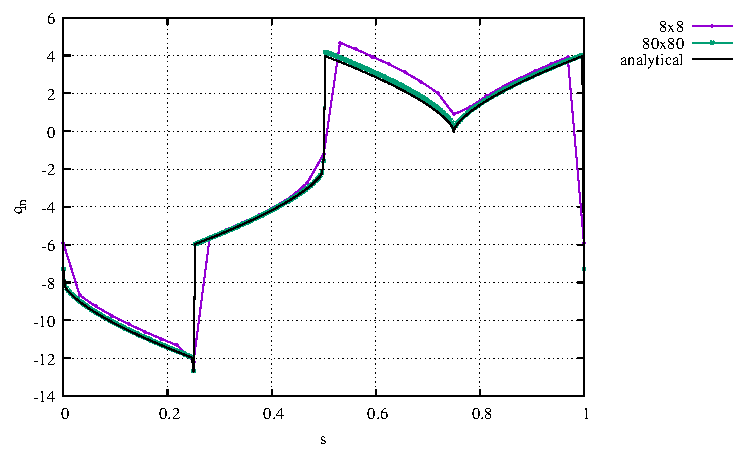
\includegraphics[width=8.5cm]{python_codes/fieldstone_173/results/heat_flux_boundary.pdf}
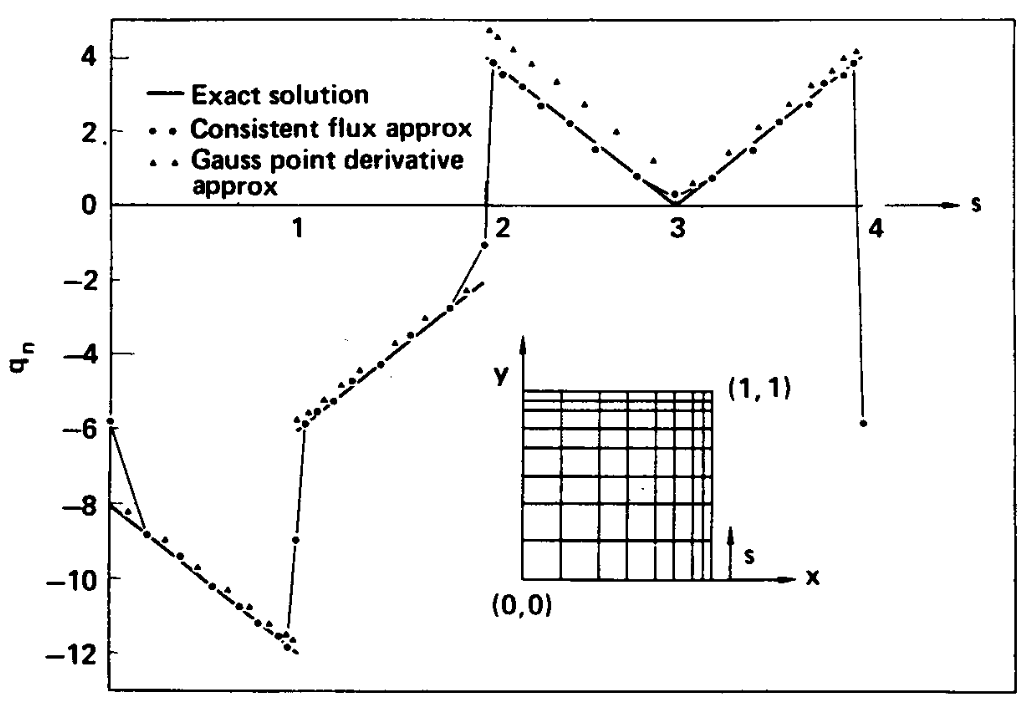
\includegraphics[width=7.5cm]{python_codes/fieldstone_173/images/grls87a}\\
{\captionfont Rather annoyingly the figure of the paper is poorly digitized 
to the point that it is somewhat dificult to distinguish between dots and triangles data points.}
\end{center}

These observations motivate the following section.
Also, this problem is not new and we read in \textcite{mizu86} (1986):
\begin{displayquote}
Most finite element schemes for thermal problems estimate boundary heat flux directly from the
derivative of the finite element solution. The boundary flux calculated by this approach is typically
inaccurate and does not guarantee a global heat balance.
\end{displayquote}

%==============================================================================
\section*{Computing the boundary heat flux}

In \textcite{mizu86} (1986) we find\footnote{I have replaced $\phi$ by $T$ and 
the source term $f$ by $S$.}
\[
\sum_{k \in \Gamma_g} \int_{\Gamma_g} \bN_i \bN_k d\Gamma \; 
\left(
\frac{\partial T}{\partial n}
\right)_k
=
\int_\Omega \vec\nabla \bN_i \cdot \vec\nabla T^h \; d\Omega
- \int_\Omega \bN_i S \; d\Omega
\qquad
i \in \Gamma_g
\]
where $T^h$ is the computed temperature and $\Gamma_g$ is the part of the 
boundary where Dirichelt boundary conditions are imposed.

Let us first consider a very simple case of a $3\times 2$ mesh:

\begin{verbatim}
8----9---10---11
| 3  | 4  | 5  |
4----5----6----7
| 0  | 1  | 2  |
0----1----2----3   Gamma_g={y=0} = nodes 0,1,2,3
\end{verbatim}



We start from 
\begin{equation}
\sum_{k \in \Gamma_g} \int_{\Gamma_g} \bN_i \bN_k d\Gamma \; 
\left(
\frac{\partial T}{\partial n}
\right)_k
=
\int_\Omega \vec\nabla \bN_i \cdot \vec\nabla T^h \; d\Omega
- \int_\Omega \bN_i S \; d\Omega
\qquad
i \in \Gamma_g
\label{eq:mizu1}
\end{equation}

First, looking at the figure above, we identify nodes 0,1,2,3 as 
being part of $\Gamma_g$, so $i=1,2,3,4$. Likewise the sum over $k$ 
runs over $k=0,1,2,3$.

We define $q_k= -\left(\frac{\partial T}{\partial n}\right)_k$ 
(assuming the heat conductivity $k=1$) 
so that now:
\[
\sum_{k \in \Gamma_g} \int_{\Gamma_g} \bN_i \bN_k d\Gamma \; 
q_k
=
-\int_\Omega \vec\nabla \bN_i \cdot \vec\nabla T^h \; d\Omega
+ \int_\Omega \bN_i S \; d\Omega
\qquad
i \in \Gamma_g
\]


Let us consider the left hand side of the equation:
\begin{eqnarray}
LHS_i= \sum_{k \in \Gamma_g} \int_{\Gamma_g} \bN_i \bN_k d\Gamma \; q_k
&=&
\int_{\Gamma_g} \bN_i \bN_0 d\Gamma \; q_0 +
\int_{\Gamma_g} \bN_i \bN_1 d\Gamma \; q_1 +
\int_{\Gamma_g} \bN_i \bN_2 d\Gamma \; q_2 +
\int_{\Gamma_g} \bN_i \bN_3 d\Gamma \; q_3 \nn
\end{eqnarray}

At this stage we must remember that the basis functions $\bN_i$ are non zero only
in elements to which node $i$ belongs. For example $\bN_1\bN_3=0$ since the two 
functions compact support do not overlap. 
Also we will denote by $\Gamma_{ij}$ the part of $\Gamma_g$ made of the segment
between nodes $i$ and $j$. We will make use of this in what follows.



Let us write this for $i=0,1,2,3$:

\begin{itemize}
\item $i=0$
\begin{eqnarray}
LHS_0
&=&
\int_{\Gamma_g} \bN_0 \bN_0 d\Gamma \; q_0 +
\int_{\Gamma_g} \bN_0 \bN_1 d\Gamma \; q_1 +
\int_{\Gamma_g} \bN_0 \bN_2 d\Gamma \; q_2 +
\int_{\Gamma_g} \bN_0 \bN_3 d\Gamma \; q_3 \nn\\
&=&
\int_{\Gamma_{01}} \bN_0 \bN_0 d\Gamma \; q_0 +
\int_{\Gamma_{01}} \bN_0 \bN_1 d\Gamma \; q_1 +
0 +
0 \nn
\end{eqnarray}



\item $i=1$
\begin{eqnarray}
LHS_1
&=&
\int_{\Gamma_g} \bN_1 \bN_0 d\Gamma \; q_0 +
\int_{\Gamma_g} \bN_1 \bN_1 d\Gamma \; q_1 +
\int_{\Gamma_g} \bN_1 \bN_2 d\Gamma \; q_2 +
\int_{\Gamma_g} \bN_1 \bN_3 d\Gamma \; q_3 \nn\\
&=&
\int_{\Gamma_{01}} \bN_1 \bN_0 d\Gamma \; q_0 +
\int_{\Gamma_{01}+\Gamma_{12}} \bN_1 \bN_1 d\Gamma \; q_1 +
\int_{\Gamma_{12}} \bN_1 \bN_2 d\Gamma \; q_2 +
0 \nn
\end{eqnarray}

\item $i=2$
\begin{eqnarray}
LHS_2
&=&
\int_{\Gamma_g} \bN_2 \bN_0 d\Gamma \; q_0 +
\int_{\Gamma_g} \bN_2 \bN_1 d\Gamma \; q_1 +
\int_{\Gamma_g} \bN_2 \bN_2 d\Gamma \; q_2 +
\int_{\Gamma_g} \bN_2 \bN_3 d\Gamma \; q_3 \nn\\
&=&
0+
\int_{\Gamma_{12}} \bN_2 \bN_1 d\Gamma \; q_1 +
\int_{\Gamma_{12}+\Gamma_{23}} \bN_2 \bN_2 d\Gamma \; q_2 +
\int_{\Gamma_{23}} \bN_2 \bN_3 d\Gamma \; q_3 \nn
\end{eqnarray}



\item $i=3$
\begin{eqnarray}
LHS_3
&=&
\int_{\Gamma_g} \bN_3 \bN_0 d\Gamma \; q_0 +
\int_{\Gamma_g} \bN_3 \bN_1 d\Gamma \; q_1 +
\int_{\Gamma_g} \bN_3 \bN_2 d\Gamma \; q_2 +
\int_{\Gamma_g} \bN_3 \bN_3 d\Gamma \; q_3 \nn\\
&=&
0 +
0 +
\int_{\Gamma_{23}} \bN_3 \bN_2 d\Gamma \; q_2 +
\int_{\Gamma_{23}} \bN_3 \bN_3 d\Gamma \; q_3 \nn
\end{eqnarray}

\end{itemize}


The 2d basis functions (in the reference element) $\bN$ are functions of $r$ and $s$.
However in this case nodes 0,1,2,3 are on the bottom face of each element and correspond
to $s=-1$ so that the basis functions under consideration are only functions of $r$ on $\Gamma_g$.
Looking at the integrals above we have to compute three types of integrals:
\[
\int_{\Gamma_{m,m+1}} \bN_m\bN_{m+1} d\Gamma,
\qquad
\int_{\Gamma_{m-1,m}} \bN_m\bN_m d\Gamma
\qquad
\text{and}
\qquad
\int_{\Gamma_{m,m+1}} \bN_m\bN_m d\Gamma
\]
In what follows we assume that all elements have the same size $h_x$ for simplicity so that 
the Jacobian of the change of variables $x \rightarrow r$ is simply $h_x/2$.
Then
\[
\int_{\Gamma_{m,m+1}} \bN_m\bN_{m+1} d\Gamma 
= \frac{h_x}{2} \int_{-1}^{+1} \frac12 (1-r) \frac12(1+r) dr 
= \frac{h_x}{6}
\]
\[
\int_{\Gamma_{m-1,n}} \bN_m\bN_m d\Gamma
= \frac{h_x}{2} \int_{-1}^{+1} \frac12 (1+r) \frac12(1+r) dr 
= \frac{h_x}{3}
\]
\[
\int_{\Gamma_{m,m+1}} \bN_m\bN_m d\Gamma
= \frac{h_x}{2} \int_{-1}^{+1} \frac12 (1-r) \frac12(1-r) dr 
= \frac{h_x}{3}
\]

In the end we arrive at
\begin{eqnarray}
LHS_0 &=&  \frac{h_x}{3} q_0 + \frac{h_x}{6} q_1 \nn\\  
LHS_1 &=&  \frac{h_x}{6} q_0 + \frac{2h_x}{3} q_1  + \frac{h_x}{6} q_2  \nn\\
LHS_2 &=&  \frac{h_x}{6} q_1 + \frac{2h_x}{3} q_2  + \frac{h_x}{6} q_3  \nn\\
LHS_3 &=&  \frac{h_x}{6} q_2  +\frac{h_x}{3} q_3  \nn
\end{eqnarray}




We can now turn to the right hand side of Eq.~\eqref{eq:mizu1}:
\[
RHS_i=
-\int_\Omega \vec\nabla \bN_i \cdot \vec\nabla T^h \; d\Omega
+ \int_\Omega \bN_i S \; d\Omega
\]
Since $i=0,1,2,3$ are on the boundary and since the basis functions 
have compact support then the integrals $\int_\Omega$ become integrals 
over elements that are on the bottom boundary of the domain. 
In what follows we denote by $\Omega_e$ the element $e$.

\begin{itemize}
\item $i=0$:
\begin{eqnarray}
RHS_0 
&=& -\int_{\Omega_0} \vec\nabla \bN_0 \cdot \vec\nabla T^h \; d\Omega + \int_{\Omega_0} \bN_0 S \; d\Omega
\end{eqnarray}

\item $i=1$:
\begin{eqnarray}
RHS_1
&=& -\int_{\Omega_0+\Omega_1} \vec\nabla \bN_1 \cdot \vec\nabla T^h \; d\Omega + \int_{\Omega_0+\Omega_1} \bN_1 S \; d\Omega
\end{eqnarray}

\item $i=2$:
\begin{eqnarray}
RHS_2
&=& -\int_{\Omega_1+\Omega_2} \vec\nabla \bN_2 \cdot \vec\nabla T^h \; d\Omega + \int_{\Omega_1+\Omega_2} \bN_2 S \; d\Omega
\end{eqnarray}

\item $i=3$:
\begin{eqnarray}
RHS_3
&=& -\int_{\Omega_2} \vec\nabla \bN_3 \cdot \vec\nabla T^h \; d\Omega + \int_{\Omega_2} \bN_3 S \; d\Omega
\end{eqnarray}

\end{itemize}




These integrals are simple to compute and pose no real problem. 
In the end we have 4 equations and 4 unknowns $q_0,q_1,q_2,q_3$.
This can be cast as a linear system:
\begin{equation}
\underbrace{
\left(
\begin{array}{cccc}
h_x/3 & h_x/6  &  0 & 0\\
h_x/6 & 2h_x/3  & h_x/6  & 0\\
0 & h_x/6  & 2h_x/3  & h_x/6 \\ 
0 & 0  &  h_x/6 & h_x/3
\end{array}
\right)
}_{M}
\cdot
\underbrace{
\left(
\begin{array}{c}
q_0 \\ q_1 \\ q_2 \\ q_3
\end{array}
\right)
}_{\vec{q}}
=
\underbrace{
\left(
\begin{array}{c}
RHS_0 \\ RHS_1 \\ RHS_2 \\ RHS_3
\end{array}
\right)
}_{\vec{f}}
\label{eq:mizu2}
\end{equation}
This is obviously the 1d mass matrix obtained from the bottom boundary of the domain,
see appendix XXX.



\paragraph{A note about lumping} If we lump the matrix we obtain:
\begin{equation}
\underbrace{\left(
\begin{array}{cccc}
h_x/2 & 0  &  0 & 0\\
0 & h_x  & 0  & 0\\
0 & 0  & h_x  & 0 \\ 
0 & 0  &  0 & h_x/2
\end{array}
\right)}_{M_l}
\cdot
\underbrace{
\left(
\begin{array}{c}
q_0 \\ q_1 \\ q_2 \\ q_3
\end{array}
\right)
}_{\vec{q}}
=
\underbrace{
\left(
\begin{array}{c}
RHS_0 \\ RHS_1 \\ RHS_2 \\ RHS_3
\end{array}
\right)}_{\vec{f}}
\label{eq:mizu3}
\end{equation}
In this case the solution is then simply:
\[
\vec{q} = M_l^{-1} \cdot \vec{f}
=\frac{1}{h_x}
\left(
\begin{array}{c}
2RHS_0 \\ RHS_1 \\ RHS_2 \\ 2RHS_3
\end{array}
\right)
\]



Let us now consider the mesh (topology) of \textcite{grls87}:
\begin{center}
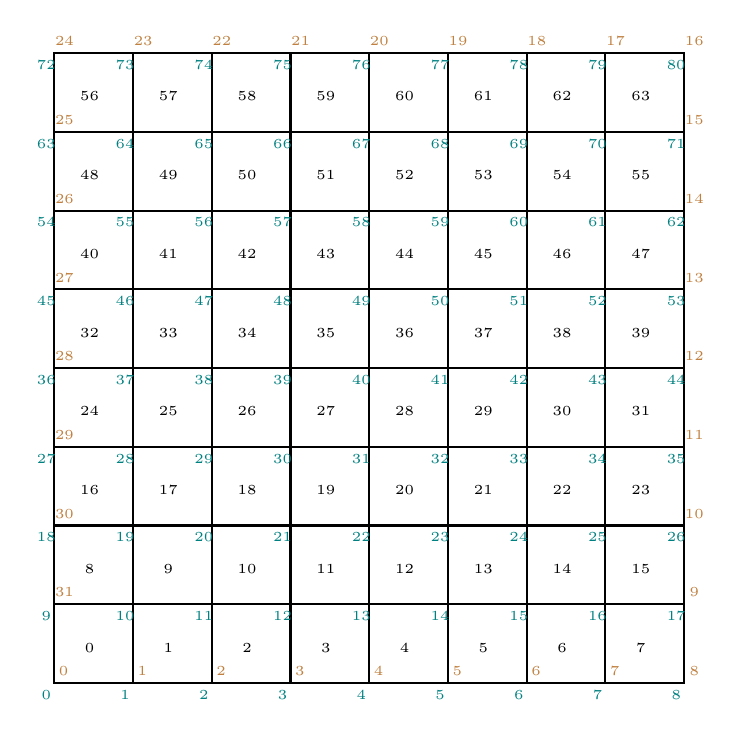
\begin{tikzpicture}
%\draw[step=0.5cm,gray,very thin] (0,0) grid (10,10); %background grid

\draw[thick] (0,0)--(8,0)--(8,8)--(0,8)--cycle;  

\draw[thick] (0,1)--(8,1);  
\draw[thick] (0,2)--(8,2);  
\draw[thick] (0,3)--(8,3);  
\draw[thick] (0,4)--(8,4);  
\draw[thick] (0,5)--(8,5);  
\draw[thick] (0,6)--(8,6);  
\draw[thick] (0,7)--(8,7);  
\draw[thick] (0,8)--(8,8);  

\draw[thick] (1,0)--(1,8);  
\draw[thick] (2,0)--(2,8);  
\draw[thick] (3,0)--(3,8);  
\draw[thick] (4,0)--(4,8);  
\draw[thick] (5,0)--(5,8);  
\draw[thick] (6,0)--(6,8);  
\draw[thick] (7,0)--(7,8);  
\draw[thick] (8,0)--(8,8);  

%%%%%%%%%%%%%%%%%%%%%%%%%%%%%%%%%%%% element numbers

\node[] at (0.45,0.45) {\tiny 0};
\node[] at (1.45,0.45) {\tiny 1};
\node[] at (2.45,0.45) {\tiny 2};
\node[] at (3.45,0.45) {\tiny 3};
\node[] at (4.45,0.45) {\tiny 4};
\node[] at (5.45,0.45) {\tiny 5};
\node[] at (6.45,0.45) {\tiny 6};
\node[] at (7.45,0.45) {\tiny 7};

\node[] at (0.45,1.45) {\tiny 8};
\node[] at (1.45,1.45) {\tiny 9};
\node[] at (2.45,1.45) {\tiny 10};
\node[] at (3.45,1.45) {\tiny 11};
\node[] at (4.45,1.45) {\tiny 12};
\node[] at (5.45,1.45) {\tiny 13};
\node[] at (6.45,1.45) {\tiny 14};
\node[] at (7.45,1.45) {\tiny 15};

\node[] at (0.45,2.45) {\tiny 16};
\node[] at (1.45,2.45) {\tiny 17};
\node[] at (2.45,2.45) {\tiny 18};
\node[] at (3.45,2.45) {\tiny 19};
\node[] at (4.45,2.45) {\tiny 20};
\node[] at (5.45,2.45) {\tiny 21};
\node[] at (6.45,2.45) {\tiny 22};
\node[] at (7.45,2.45) {\tiny 23};

\node[] at (0.45,3.45) {\tiny 24};
\node[] at (1.45,3.45) {\tiny 25};
\node[] at (2.45,3.45) {\tiny 26};
\node[] at (3.45,3.45) {\tiny 27};
\node[] at (4.45,3.45) {\tiny 28};
\node[] at (5.45,3.45) {\tiny 29};
\node[] at (6.45,3.45) {\tiny 30};
\node[] at (7.45,3.45) {\tiny 31};

\node[] at (0.45,4.45) {\tiny 32};
\node[] at (1.45,4.45) {\tiny 33};
\node[] at (2.45,4.45) {\tiny 34};
\node[] at (3.45,4.45) {\tiny 35};
\node[] at (4.45,4.45) {\tiny 36};
\node[] at (5.45,4.45) {\tiny 37};
\node[] at (6.45,4.45) {\tiny 38};
\node[] at (7.45,4.45) {\tiny 39};

\node[] at (0.45,5.45) {\tiny 40};
\node[] at (1.45,5.45) {\tiny 41};
\node[] at (2.45,5.45) {\tiny 42};
\node[] at (3.45,5.45) {\tiny 43};
\node[] at (4.45,5.45) {\tiny 44};
\node[] at (5.45,5.45) {\tiny 45};
\node[] at (6.45,5.45) {\tiny 46};
\node[] at (7.45,5.45) {\tiny 47};

\node[] at (0.45,6.45) {\tiny 48};
\node[] at (1.45,6.45) {\tiny 49};
\node[] at (2.45,6.45) {\tiny 50};
\node[] at (3.45,6.45) {\tiny 51};
\node[] at (4.45,6.45) {\tiny 52};
\node[] at (5.45,6.45) {\tiny 53};
\node[] at (6.45,6.45) {\tiny 54};
\node[] at (7.45,6.45) {\tiny 55};

\node[] at (0.45,7.45) {\tiny 56};
\node[] at (1.45,7.45) {\tiny 57};
\node[] at (2.45,7.45) {\tiny 58};
\node[] at (3.45,7.45) {\tiny 59};
\node[] at (4.45,7.45) {\tiny 60};
\node[] at (5.45,7.45) {\tiny 61};
\node[] at (6.45,7.45) {\tiny 62};
\node[] at (7.45,7.45) {\tiny 63};

%%%%%%%%%%%%%%%%%%%%%%%%%%%%%%%%%%%% nodes

\node[] at (-0.1,-0.15) {\color{teal} \tiny 0};
\node[] at (0.9,-0.15) {\color{teal} \tiny 1};
\node[] at (1.9,-0.15) {\color{teal} \tiny 2};
\node[] at (2.9,-0.15) {\color{teal} \tiny 3};
\node[] at (3.9,-0.15) {\color{teal} \tiny 4};
\node[] at (4.9,-0.15) {\color{teal} \tiny 5};
\node[] at (5.9,-0.15) {\color{teal} \tiny 6};
\node[] at (6.9,-0.15) {\color{teal} \tiny 7};
\node[] at (7.9,-0.15) {\color{teal} \tiny 8};

\node[] at (-0.1,0.85) {\color{teal} \tiny 9};
\node[] at (0.9,0.85) {\color{teal} \tiny 10};
\node[] at (1.9,0.85) {\color{teal} \tiny 11};
\node[] at (2.9,0.85) {\color{teal} \tiny 12};
\node[] at (3.9,0.85) {\color{teal} \tiny 13};
\node[] at (4.9,0.85) {\color{teal} \tiny 14};
\node[] at (5.9,0.85) {\color{teal} \tiny 15};
\node[] at (6.9,0.85) {\color{teal} \tiny 16};
\node[] at (7.9,0.85) {\color{teal} \tiny 17};

\node[] at (-0.1,1.85) {\color{teal} \tiny 18};
\node[] at (0.9,1.85) {\color{teal} \tiny 19};
\node[] at (1.9,1.85) {\color{teal} \tiny 20};
\node[] at (2.9,1.85) {\color{teal} \tiny 21};
\node[] at (3.9,1.85) {\color{teal} \tiny 22};
\node[] at (4.9,1.85) {\color{teal} \tiny 23};
\node[] at (5.9,1.85) {\color{teal} \tiny 24};
\node[] at (6.9,1.85) {\color{teal} \tiny 25};
\node[] at (7.9,1.85) {\color{teal} \tiny 26};

\node[] at (-0.1,2.85) {\color{teal} \tiny 27};
\node[] at (0.9,2.85) {\color{teal} \tiny 28};
\node[] at (1.9,2.85) {\color{teal} \tiny 29};
\node[] at (2.9,2.85) {\color{teal} \tiny 30};
\node[] at (3.9,2.85) {\color{teal} \tiny 31};
\node[] at (4.9,2.85) {\color{teal} \tiny 32};
\node[] at (5.9,2.85) {\color{teal} \tiny 33};
\node[] at (6.9,2.85) {\color{teal} \tiny 34};
\node[] at (7.9,2.85) {\color{teal} \tiny 35};

\node[] at (-0.1,3.85) {\color{teal} \tiny 36};
\node[] at (0.9,3.85) {\color{teal} \tiny 37};
\node[] at (1.9,3.85) {\color{teal} \tiny 38};
\node[] at (2.9,3.85) {\color{teal} \tiny 39};
\node[] at (3.9,3.85) {\color{teal} \tiny 40};
\node[] at (4.9,3.85) {\color{teal} \tiny 41};
\node[] at (5.9,3.85) {\color{teal} \tiny 42};
\node[] at (6.9,3.85) {\color{teal} \tiny 43};
\node[] at (7.9,3.85) {\color{teal} \tiny 44};

\node[] at (-0.1,4.85) {\color{teal} \tiny 45};
\node[] at (0.9,4.85) {\color{teal} \tiny 46};
\node[] at (1.9,4.85) {\color{teal} \tiny 47};
\node[] at (2.9,4.85) {\color{teal} \tiny 48};
\node[] at (3.9,4.85) {\color{teal} \tiny 49};
\node[] at (4.9,4.85) {\color{teal} \tiny 50};
\node[] at (5.9,4.85) {\color{teal} \tiny 51};
\node[] at (6.9,4.85) {\color{teal} \tiny 52};
\node[] at (7.9,4.85) {\color{teal} \tiny 53};

\node[] at (-0.1,5.85) {\color{teal} \tiny 54};
\node[] at (0.9,5.85) {\color{teal} \tiny 55};
\node[] at (1.9,5.85) {\color{teal} \tiny 56};
\node[] at (2.9,5.85) {\color{teal} \tiny 57};
\node[] at (3.9,5.85) {\color{teal} \tiny 58};
\node[] at (4.9,5.85) {\color{teal} \tiny 59};
\node[] at (5.9,5.85) {\color{teal} \tiny 60};
\node[] at (6.9,5.85) {\color{teal} \tiny 61};
\node[] at (7.9,5.85) {\color{teal} \tiny 62};

\node[] at (-0.1,6.85) {\color{teal} \tiny 63};
\node[] at (0.9,6.85) {\color{teal} \tiny 64};
\node[] at (1.9,6.85) {\color{teal} \tiny 65};
\node[] at (2.9,6.85) {\color{teal} \tiny 66};
\node[] at (3.9,6.85) {\color{teal} \tiny 67};
\node[] at (4.9,6.85) {\color{teal} \tiny 68};
\node[] at (5.9,6.85) {\color{teal} \tiny 69};
\node[] at (6.9,6.85) {\color{teal} \tiny 70};
\node[] at (7.9,6.85) {\color{teal} \tiny 71};

\node[] at (-0.1,7.85) {\color{teal} \tiny 72};
\node[] at (0.9,7.85) {\color{teal} \tiny 73};
\node[] at (1.9,7.85) {\color{teal} \tiny 74};
\node[] at (2.9,7.85) {\color{teal} \tiny 75};
\node[] at (3.9,7.85) {\color{teal} \tiny 76};
\node[] at (4.9,7.85) {\color{teal} \tiny 77};
\node[] at (5.9,7.85) {\color{teal} \tiny 78};
\node[] at (6.9,7.85) {\color{teal} \tiny 79};
\node[] at (7.9,7.85) {\color{teal} \tiny 80};


%%%%%%%%%%%%%%%%%%%%%%%%%%%%%%%%%%%% B nodes

\node[] at (0.12,0.15) {\color{brown} \tiny 0};
\node[] at (1.12,0.15) {\color{brown} \tiny 1};
\node[] at (2.12,0.15) {\color{brown} \tiny 2};
\node[] at (3.12,0.15) {\color{brown} \tiny 3};
\node[] at (4.12,0.15) {\color{brown} \tiny 4};
\node[] at (5.12,0.15) {\color{brown} \tiny 5};
\node[] at (6.12,0.15) {\color{brown} \tiny 6};
\node[] at (7.12,0.15) {\color{brown} \tiny 7};

\node[] at (8.13,0.15) {\color{brown} \tiny 8};
\node[] at (8.13,1.15) {\color{brown} \tiny 9};
\node[] at (8.13,2.15) {\color{brown} \tiny 10};
\node[] at (8.13,3.15) {\color{brown} \tiny 11};
\node[] at (8.13,4.15) {\color{brown} \tiny 12};
\node[] at (8.13,5.15) {\color{brown} \tiny 13};
\node[] at (8.13,6.15) {\color{brown} \tiny 14};
\node[] at (8.13,7.15) {\color{brown} \tiny 15};
\node[] at (8.13,8.15) {\color{brown} \tiny 16};

\node[] at (0.13,8.15) {\color{brown} \tiny 24};
\node[] at (1.13,8.15) {\color{brown} \tiny 23};
\node[] at (2.13,8.15) {\color{brown} \tiny 22};
\node[] at (3.13,8.15) {\color{brown} \tiny 21};
\node[] at (4.13,8.15) {\color{brown} \tiny 20};
\node[] at (5.13,8.15) {\color{brown} \tiny 19};
\node[] at (6.13,8.15) {\color{brown} \tiny 18};
\node[] at (7.13,8.15) {\color{brown} \tiny 17};

\node[] at (0.13,7.15) {\color{brown} \tiny 25};
\node[] at (0.13,6.15) {\color{brown} \tiny 26};
\node[] at (0.13,5.15) {\color{brown} \tiny 27};
\node[] at (0.13,4.15) {\color{brown} \tiny 28};
\node[] at (0.13,3.15) {\color{brown} \tiny 29};
\node[] at (0.13,2.15) {\color{brown} \tiny 30};
\node[] at (0.13,1.15) {\color{brown} \tiny 31};

\end{tikzpicture}
\end{center}





The number of nodes on the $\Gamma_g$ boundary is the total
number of nodes on the boundary, i.e. \lstinline{NB=(nelx+nely)*2=32} in this case 
since $\Gamma_h=0$.

For the purpose of the implementation we will need two boolean arrays
\lstinline{boundary_node} and \lstinline{boundary_element}.

\begin{lstlisting}
boundary_element=np.zeros(nel,dtype=bool)  
boundary_node=np.zeros(NV,dtype=bool)  

counter=0
for j in range(0,nely):
    for i in range(0,nelx):
        if i==0 or i==nelx-1 or j==0 or j==nely-1: 
           boundary_element[counter]=True 
        counter+=1

counter=0
for j in range(0,nny):
    for i in range(0,nnx):
        if i==0 or i==nnx-1 or j==0 or j==nny-1: 
           boundary_node[counter]=True 
        counter+=1
\end{lstlisting}

Furthermore we will also need an array which associates to 
boundary nodes their {\color{teal} global domain number} (between 0 and 80)
with their {\color{teal} boundary number} (between 0 and 31).

The array \lstinline{B_to_G} ('boundary to global') 
of size \lstinline{NB} is filled with
\begin{lstlisting}
[ 0  1  2  3  4  5  6  7  8 17 26 35 44 53 62 71 80 79 78 77 76 75 74 73
 72 63 54 45 36 27 18  9]
\end{lstlisting}
It maps the {\color{brown} boundary nodes} (0 to 31) 
to their {\color{teal} global number} (0 to 80).
Likewise the array \lstinline{G_to_B} is of size \lstinline{N} 
and is equal to -1 if the node in not on the boundary and equal 
to the  {\color{brown} boundary number} if the node lies on the boundary

The code is as follows:
\begin{lstlisting}
NB=2*(nelx+nely)

B_to_G=np.zeros((NB),dtype=np.int32) ; B_to_G[:]=-1
G_to_B=np.zeros((NV),dtype=np.int32) ; G_to_B[:]=-1

counter=0
for i in range(0,nnx): 
        inode=i
        G_to_B[inode]=counter
        B_to_G[counter]=inode
        counter+=1
counter-=1
for i in range(0,nny):
        inode=nnx*(i+1)-1
        G_to_B[inode]=counter
        B_to_G[counter]=inode
        counter+=1
counter-=1
for i in range(0,nnx): 
        inode=NV-i-1
        G_to_B[inode]=counter
        B_to_G[counter]=inode
        counter+=1
counter-=1
for i in range(0,nny-1):
        inode=NV-(i+1)*nnx
        G_to_B[inode]=counter
        B_to_G[counter]=inode
        counter+=1
\end{lstlisting}





For the implementation of the CBF itself, one could then loop over
all the boundary nodes ($i=0,31$), compute $LHS_i$ and $RHS_i$, 
and fill the corresponding line in the matrix and right hand side vector.
However, the simple example above did not address the case of corner nodes
when the belong to two faces.
Also, the matrix above was arrived at assuming all elements to be of equal size. 
Let us now rewrite the matrix above as

\[
\left(
\begin{array}{cccc}
h_x/3 & h_x/6  &  0 & 0\\
h_x/6 & 2h_x/3  & h_x/6  & 0\\
0 & h_x/6  & 2h_x/3  & h_x/6 \\ 
0 & 0  &  h_x/6 & h_x/3
\end{array}
\right)
=
\left(
\begin{array}{cccc}
h_x/3 & h_x/6  &  0 & 0\\
h_x/6 & h_x/3  & 0  & 0\\
0 & 0  & 0  & 0 \\ 
0 & 0  &  0 & 0
\end{array}
\right)
+
\left(
\begin{array}{cccc}
0 & 0  &  0 & 0\\
0 & h_x/3  & h_x/6  & 0\\
0 & h_x/6  & h_x/3  & 0 \\ 
0 & 0  &  0 & 0
\end{array}
\right)
+
\left(
\begin{array}{cccc}
0 & 0  &  0 & 0\\
0 & 0  & 0 & 0\\
0 & 0 & h_x/3  & h_x/6 \\ 
0 & 0  &  h_x/6 & h_x/3
\end{array}
\right)
\]
We see that this follows the standard procedure of elemental assembly.
The first matrix is the mass matrix for the segment $\Gamma_{01}$ belonging to element $\Omega_0$,
the second matrix is the mass matrix for the segment $\Gamma_{12}$ belonging to element $\Omega_1$,
and the third is the mass matrix for the segment $\Gamma_{23}$ belonging to element $\Omega_2$.

Likewise the rhs vector of the linear system can be decomposed as follows
\begin{small}
\[
\left(
\begin{array}{c}
RHS_0 \\ RHS_1 \\ RHS_2 \\ RHS_3
\end{array}
\right)
=
\left(
\begin{array}{c}
\int_{\Omega_0} \vec\nabla \bN_0 \cdot \vec\nabla T^h \; d\Omega - \int_{\Omega_0} \bN_0 S \; d\Omega \\
\int_{\Omega_0} \vec\nabla \bN_1 \cdot \vec\nabla T^h \; d\Omega - \int_{\Omega_0} \bN_1 S \; d\Omega \\
0 \\ 0
\end{array}
\right)
+
\left(
\begin{array}{c}
0 \\
\int_{\Omega_1} \vec\nabla \bN_1 \cdot \vec\nabla T^h \; d\Omega - \int_{\Omega_1} \bN_1 S \; d\Omega \\
\int_{\Omega_1} \vec\nabla \bN_2 \cdot \vec\nabla T^h \; d\Omega - \int_{\Omega_1} \bN_2 S \; d\Omega \\
0
\end{array}
\right)
+
\left(
\begin{array}{c}
0 \\ 0 \\
\int_{\Omega_2} \vec\nabla \bN_2 \cdot \vec\nabla T^h \; d\Omega - \int_{\Omega_2} \bN_2 S \; d\Omega\\
\int_{\Omega_2} \vec\nabla \bN_3 \cdot \vec\nabla T^h \; d\Omega - \int_{\Omega_2} \bN_3 S \; d\Omega
\end{array}
\right)
\]

\end{small}
We see that the rhs of the linear system is also the result of an element-by-element-based assembly process.


For a given node edge made of nodes $k-l$ of length $h$ we will need to build
the following elemental matrix and rhs:
\[
\left(
\begin{array}{cc}
h/3 & h/6  \\
h/6 & h/3 
\end{array}
\right)
\qquad
\text{and}
\qquad
\left(
\begin{array}{c}
\int_{\Omega_e} \vec\nabla \bN_k \cdot \vec\nabla T^h \; d\Omega - \int_{\Omega_e} \bN_k S \; d\Omega \\
\int_{\Omega_e} \vec\nabla \bN_l \cdot \vec\nabla T^h \; d\Omega - \int_{\Omega_e} \bN_l S \; d\Omega 
\end{array}
\right)
\qquad
\text{with} \; kl \in \Omega_e
\]

Note that the first term of the rhs could also have been written $\int B^T B d\Omega \cdot \vec{T}^h$.




\paragraph{Implementation} We start by declaring the required arrays:
\begin{lstlisting}
    M=lil_matrix((NB,NB),dtype=np.float64)
    Ml=lil_matrix((NB,NB),dtype=np.float64)
    rhs= np.zeros(NB,dtype=np.float64)   
    Mel=np.zeros((2,2),dtype=np.float64) 
\end{lstlisting}

Then we proceed as follows:

\begin{lstlisting}
    for iel in range(0,nel):
        if boundary_element[iel]:
           for face in range(0,4): # loop over faces
               k=face    ; inode=icon[k,iel]
               l=(k+1)%4 ; jnode=icon[l,iel]
               if boundary_node[inode] and boundary_node[jnode]: # both nodes are on boundary
                  if bc_fixT[inode] and bc_fixT[jnode]: # both nodes are fixed

                     print('iel=',iel,'face=',face,'k=',k,'l=',l,'inode=',inode,'jnode=',jnode,
                             'h=',h,G_to_B[inode],G_to_B[jnode])

                     # compute Mel, assuming all sides are straight
                     Mel[0,0]=h/3  
                     Mel[0,1]=h/6  
                     Mel[1,0]=h/6  
                     Mel[1,1]=h/3  

                     # compute bel, integration over volume
                     bel=np.zeros(2,dtype=np.float64) 
                     for iq in range(0,nqperdim):
                         for jq in range(0,nqperdim):
                             ...
                             bel[0]-=(dNNNTdx[k]*dTdxq+dNNNTdy[k]*dTdyq)*weightq*jcob
                             bel[1]-=(dNNNTdx[l]*dTdxq+dNNNTdy[l]*dTdyq)*weightq*jcob
                             ...
                             bel[0]+=(NNNT[k]*rhs_f(xq,yq,experiment))*weightq*jcob
                             bel[1]+=(NNNT[l]*rhs_f(xq,yq,experiment))*weightq*jcob
                         #end for jq
                     #end for iq

                     #assembly                                          
                     M[G_to_B[inode],G_to_B[inode]]+=Mel[0,0]
                     M[G_to_B[inode],G_to_B[jnode]]+=Mel[0,1]
                     M[G_to_B[jnode],G_to_B[inode]]+=Mel[1,0]
                     M[G_to_B[jnode],G_to_B[jnode]]+=Mel[1,1]
                     rhs[G_to_B[inode]]+=bel[0]
                     rhs[G_to_B[jnode]]+=bel[1]

\end{lstlisting}


The print statement in the code above yields the following screen output
which allows us to verify that we are targetting the correct elements, faces, nodes, etc ...
\begin{lstlisting}
iel= 0 face= 0 k= 0 l= 1 inode= 0 jnode= 1 h= 0.125 0 1
iel= 0 face= 3 k= 3 l= 0 inode= 9 jnode= 0 h= 0.125 31 0
iel= 1 face= 0 k= 0 l= 1 inode= 1 jnode= 2 h= 0.125 1 2
iel= 2 face= 0 k= 0 l= 1 inode= 2 jnode= 3 h= 0.125 2 3
iel= 3 face= 0 k= 0 l= 1 inode= 3 jnode= 4 h= 0.125 3 4
iel= 4 face= 0 k= 0 l= 1 inode= 4 jnode= 5 h= 0.125 4 5
iel= 5 face= 0 k= 0 l= 1 inode= 5 jnode= 6 h= 0.125 5 6
iel= 6 face= 0 k= 0 l= 1 inode= 6 jnode= 7 h= 0.125 6 7
iel= 7 face= 0 k= 0 l= 1 inode= 7 jnode= 8 h= 0.125 7 8
iel= 7 face= 1 k= 1 l= 2 inode= 8 jnode= 17 h= 0.125 8 9
iel= 8 face= 3 k= 3 l= 0 inode= 18 jnode= 9 h= 0.125 30 31
iel= 15 face= 1 k= 1 l= 2 inode= 17 jnode= 26 h= 0.125 9 10
iel= 16 face= 3 k= 3 l= 0 inode= 27 jnode= 18 h= 0.125 29 30
iel= 23 face= 1 k= 1 l= 2 inode= 26 jnode= 35 h= 0.125 10 11
iel= 24 face= 3 k= 3 l= 0 inode= 36 jnode= 27 h= 0.125 28 29
iel= 31 face= 1 k= 1 l= 2 inode= 35 jnode= 44 h= 0.125 11 12
iel= 32 face= 3 k= 3 l= 0 inode= 45 jnode= 36 h= 0.125 27 28
iel= 39 face= 1 k= 1 l= 2 inode= 44 jnode= 53 h= 0.125 12 13
iel= 40 face= 3 k= 3 l= 0 inode= 54 jnode= 45 h= 0.125 26 27
iel= 47 face= 1 k= 1 l= 2 inode= 53 jnode= 62 h= 0.125 13 14
iel= 48 face= 3 k= 3 l= 0 inode= 63 jnode= 54 h= 0.125 25 26
iel= 55 face= 1 k= 1 l= 2 inode= 62 jnode= 71 h= 0.125 14 15
iel= 56 face= 2 k= 2 l= 3 inode= 73 jnode= 72 h= 0.125 23 24
iel= 56 face= 3 k= 3 l= 0 inode= 72 jnode= 63 h= 0.125 24 25
iel= 57 face= 2 k= 2 l= 3 inode= 74 jnode= 73 h= 0.125 22 23
iel= 58 face= 2 k= 2 l= 3 inode= 75 jnode= 74 h= 0.125 21 22
iel= 59 face= 2 k= 2 l= 3 inode= 76 jnode= 75 h= 0.125 20 21
iel= 60 face= 2 k= 2 l= 3 inode= 77 jnode= 76 h= 0.125 19 20
iel= 61 face= 2 k= 2 l= 3 inode= 78 jnode= 77 h= 0.125 18 19
iel= 62 face= 2 k= 2 l= 3 inode= 79 jnode= 78 h= 0.125 17 18
iel= 63 face= 1 k= 1 l= 2 inode= 71 jnode= 80 h= 0.125 15 16
iel= 63 face= 2 k= 2 l= 3 inode= 80 jnode= 79 h= 0.125 16 17
\end{lstlisting}

Once the matrix and the rhs have been built we can then solve
the linear system:

\begin{lstlisting}
    qn_CBF=sps.linalg.spsolve(sps.csr_matrix(M),rhs)
\end{lstlisting}

The lumped matrix is also built in the code above
by modifying slightly the assembly:

\begin{lstlisting}
    for iel in range(0,nel):
        if boundary_element[iel]:
           for face in range(0,4): # loop over faces
               k=face    ; inode=icon[k,iel]
               l=(k+1)%4 ; jnode=icon[l,iel]
               if boundary_node[inode] and boundary_node[jnode]: # both nodes are on boundary
                  if bc_fixT[inode] and bc_fixT[jnode]: # both nodes are fixed
                     ...
                     Ml[G_to_B[inode],G_to_B[inode]]+=Mel[0,0]
                     Ml[G_to_B[inode],G_to_B[inode]]+=Mel[0,1]
                     Ml[G_to_B[jnode],G_to_B[jnode]]+=Mel[1,0]
                     Ml[G_to_B[jnode],G_to_B[jnode]]+=Mel[1,1]
\end{lstlisting}
followed by 
\begin{lstlisting}
    qn_CBF_lumped=sps.linalg.spsolve(sps.csr_matrix(Ml),rhs)
\end{lstlisting}

We then run the code and proceed to plot
\begin{itemize}
\item the boundary heat flux \lstinline{qn} obtained by means of the averaged corner 
temperature gradients;
\item the boundary heat flux \lstinline{qn_CBF} obtained by solving a linear system as in Eq.~\eqref{eq:mizu2};
\item the boundary heat flux \lstinline{qn_CBF_lumped} obtained by solving a linear system as in Eq.~\eqref{eq:mizu3};
\item the boundary heat flux \lstinline{qn_CBF_analytical} obtained with the analytical solution and the 
computed normals above. 
\end{itemize}

Before we look at results we must acknowledge that the paper on which this all is based \cite{mizu86}
only showcases results in 1d. This observation will come to haunt us later on. 

\begin{center}
a)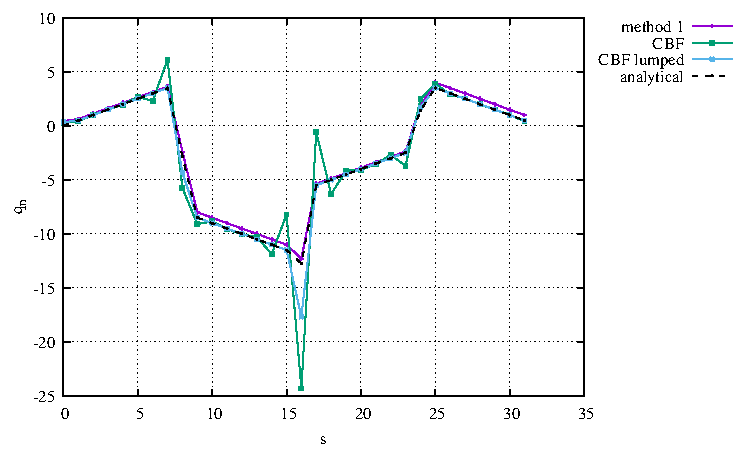
\includegraphics[width=7cm]{python_codes/fieldstone_173/results/CBF1/heat_flux_boundary.pdf}
b)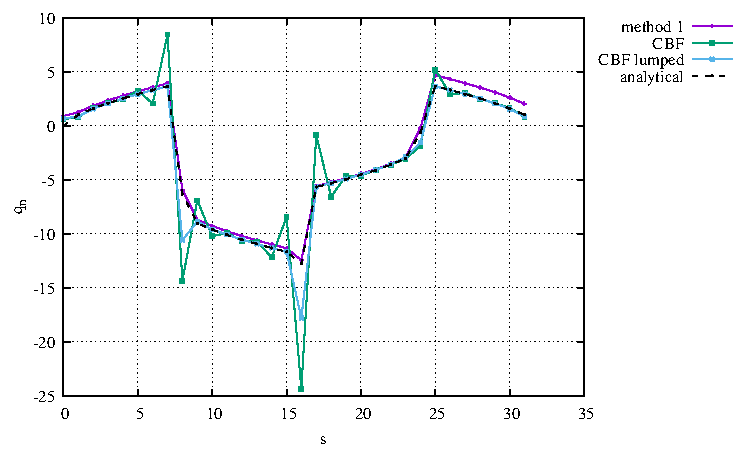
\includegraphics[width=7cm]{python_codes/fieldstone_173/results/CBF2/heat_flux_boundary.pdf}\\
c)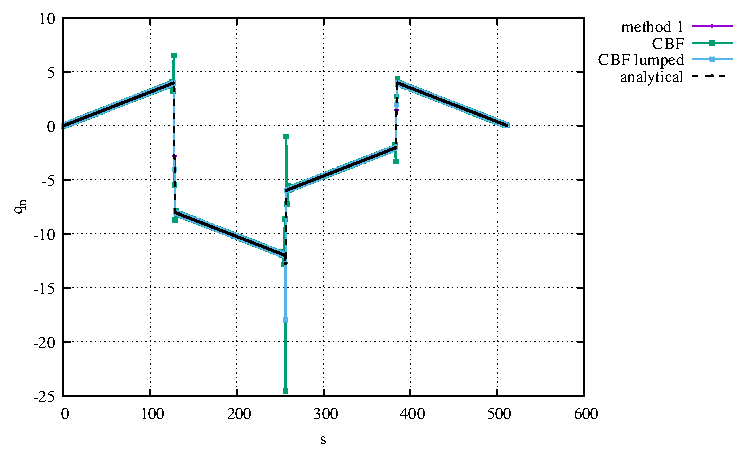
\includegraphics[width=7cm]{python_codes/fieldstone_173/results/CBF3/heat_flux_boundary.pdf}
d)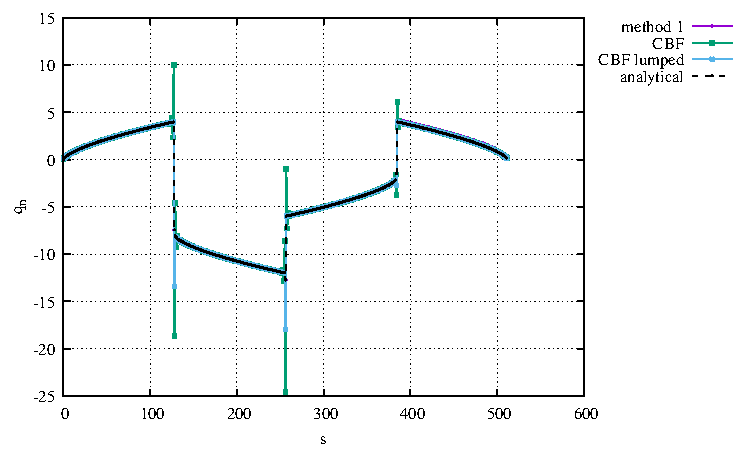
\includegraphics[width=7cm]{python_codes/fieldstone_173/results/CBF4/heat_flux_boundary.pdf}\\
{\captionfont a) \item grid $8\times 8$, no stretching; b) grid $8\times 8$, with stretching;
c) grid $128\times 128$, no stretching; d) grid $128\times 128$, with stretching. 
Note that here the measurements are done SW-SE-NE-NW-SW.}
\end{center}

The conclusion is clear: with or without stretching the CBF algorithm (lumped or not) works. 
However the presence of corners with an undefined normal yields anomalous results. 

Fortunately, this problem was also observed in Section 5 of \textcite{cacs85} (1985):
\begin{displayquote}
As noted earlier, local effects at the corners may degrade the rate of convergence of the
computed flux. Near a corner point $P$, there are two distinct unit normal vectors, each
associated with one of the two (straight line) portions of $\Gamma$. These vectors are associated with
two different limiting flux values at $P$ and hence lead to a discontinuity of the flux at the
corner. Thus if the distinct flux values at P were specified correctly one would anticipate that,
by incorporating these values in our post-processing procedures, a much more accurate flux
approximation would result.
\end{displayquote}





